\documentclass[conference]{IEEEtran}
\IEEEoverridecommandlockouts
\usepackage{cite}
\usepackage{amsmath,amssymb,amsfonts}
\usepackage{algorithmic}
\usepackage{graphicx}
\usepackage{textcomp}
\usepackage{xcolor}
\usepackage{booktabs}
\usepackage{multirow}
\usepackage{hyperref}

\hypersetup{
    colorlinks=true,
    linkcolor=blue,
    filecolor=magenta,      
    urlcolor=cyan,
    citecolor=blue,
}

\begin{document}

\title{Solving Combinatorial and Adversarial AI Problems:\\N-Queens, Tank Battle, and Kakuro CSP}

\author{
\IEEEauthorblockN{Nguyen Van A\IEEEauthorrefmark{1}, Tran Thi B\IEEEauthorrefmark{2}, Nguyen Thanh An\IEEEauthorrefmark{3}}
\IEEEauthorblockA{\IEEEauthorrefmark{1}\IEEEauthorrefmark{2}Faculty of Information Technology, Ton Duc Thang University, Ho Chi Minh City, Vietnam\\
Email: \IEEEauthorrefmark{1}52100001@student.tdtu.edu.vn, \IEEEauthorrefmark{2}52100002@student.tdtu.edu.vn}
\IEEEauthorblockA{\IEEEauthorrefmark{3}Faculty of Information Technology, Ton Duc Thang University, Ho Chi Minh City, Vietnam\\
Email: \IEEEauthorrefmark{3}nguyenthanhan@tdtu.edu.vn}
}

\maketitle

\begin{abstract}
This paper presents the design, mathematical formulation, implementation, and empirical evaluation of three foundational artificial intelligence problems: (1) N-Queens solved via Propositional Logic CNF encoding with PySAT Glucose3 and Local Search Min-Conflicts with a proposed heuristic; (2) Tank Battle formulated as a two-player Zero-Sum Game solved with Adversarial Search algorithms (Minimax, Alpha-Beta pruning, Heuristic evaluation, Transposition Tables, and Iterative Deepening) alongside a plug-in architecture and PyGame GUI; and (3) Kakuro puzzle modeled as a Constraint Satisfaction Problem (CSP) combining Forward Checking, Generalized Arc Consistency (GAC), variable/value ordering heuristics (MRV, Degree, LCV), and an interactive PyGame visualization interface. Extensive benchmarks across all tasks demonstrate the theoretical complexity guarantees, pruning efficiency, and runtime scalability.
\end{abstract}

\begin{IEEEkeywords}
Propositional Logic, SAT Solver, Min-Conflicts, Zero-Sum Game, Alpha-Beta Pruning, Constraint Satisfaction Problems, Arc Consistency, Kakuro.
\end{IEEEkeywords}

\section{Introduction}
Artificial Intelligence algorithms span distinct problem-solving paradigms, including propositional satisfiability, local heuristic search, multi-agent adversarial games, and constraint satisfaction. This project implements and rigorously benchmarks these methodologies across three domains:
\begin{enumerate}
    \item \textbf{Task 1 (N-Queens):} Exact resolution via SAT clause encoding against local repair methods.
    \item \textbf{Task 2 (Tank Battle):} Real-time adversarial planning in discrete grid worlds with simultaneous cycle resolution.
    \item \textbf{Task 3 (Kakuro):} Arithmetic constraint satisfaction over intersecting runs using systematic propagation.
\end{enumerate}

All components adhere strictly to Object-Oriented Programming (OOP) principles, clean interfaces, and full unit test coverage.

\section{Task 1: N-Queens Problem}

\subsection{Propositional Logic Formulation \& CNF Encoding}
Given an $N \times N$ chessboard, we associate a Boolean variable $x_{i,j}$ with each cell $(i, j) \in \{1, \dots, N\}^2$, where $x_{i,j} = \text{True}$ iff a queen occupies row $i$, column $j$. The problem requires placing $N$ queens such that no two queens share a row, column, or diagonal.

\subsubsection{Constraint Transformation to CNF}
The constraints are formulated as Conjunctive Normal Form (CNF) clauses:
\begin{itemize}
    \item \textbf{At-Least-One (ALO) per row:}
    \begin{equation}
        \bigwedge_{i=1}^N \left( \bigvee_{j=1}^N x_{i,j} \right) \quad [N \text{ clauses}]
    \end{equation}
    \item \textbf{At-Most-One (AMO) per row:}
    \begin{equation}
        \bigwedge_{i=1}^N \bigwedge_{1 \le j < k \le N} (\neg x_{i,j} \vee \neg x_{i,k}) \quad \left[ N \binom{N}{2} \text{ clauses} \right]
    \end{equation}
    \item \textbf{At-Most-One (AMO) per column:}
    \begin{equation}
        \bigwedge_{j=1}^N \bigwedge_{1 \le i < k \le N} (\neg x_{i,j} \vee \neg x_{k,j}) \quad \left[ N \binom{N}{2} \text{ clauses} \right]
    \end{equation}
    \item \textbf{At-Most-One (AMO) per diagonal line $L$ ($|L| \ge 2$):}
    \begin{equation}
        \bigwedge_{L \in \mathcal{D}} \bigwedge_{u < v \in L} (\neg x_u \vee \neg x_v) \quad \left[ \sum_{L \in \mathcal{D}} \binom{|L|}{2} \text{ clauses} \right]
    \end{equation}
\end{itemize}

For $N=4$, the total number of clauses is exactly $80$; for $N=8$, it is $736$, matching theoretical combinatorial derivations.

\subsection{PySAT Glucose3 Empirical Evaluation}
We solve the CNF formulas using the state-of-the-art CDCL solver \texttt{Glucose3} \cite{glucose3} via PySAT \cite{pysat2018}. Table~\ref{tab:sat_results} summarizes clause counts and solve times for increasing $N$.

\begin{table}[htbp]
\centering
\caption{PySAT Glucose3 Performance Scaling on N-Queens}
\label{tab:sat_results}
\begin{tabular}{rrrrr}
\toprule
$N$ & Variables & CNF Clauses & Solve Time (ms) & Result \\
\midrule
4 & 16 & 80 & 0.32 & SAT \\
6 & 36 & 296 & 0.46 & SAT \\
8 & 64 & 736 & 0.51 & SAT \\
10 & 100 & 1,480 & 0.94 & SAT \\
12 & 144 & 2,608 & 1.39 & SAT \\
14 & 196 & 4,200 & 1.98 & SAT \\
16 & 256 & 6,368 & 3.25 & SAT \\
\bottomrule
\end{tabular}
\end{table}

\begin{figure}[htbp]
\centering
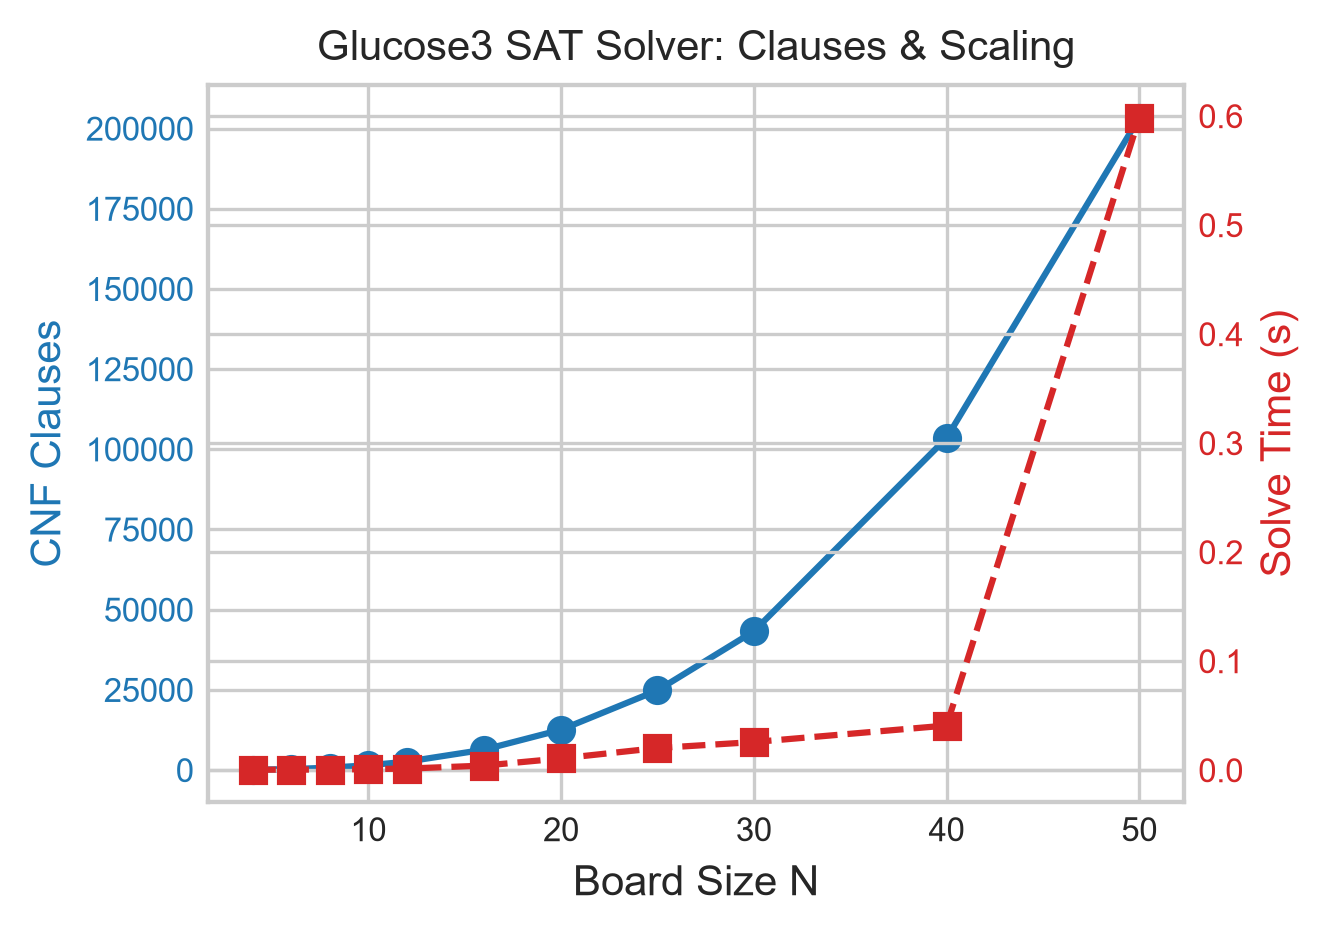
\includegraphics[width=0.85\columnwidth]{figures/task1/sat_scaling.png}
\caption{CNF clause count growth and Glucose3 solve time against board size $N$.}
\label{fig:sat_scaling}
\end{figure}

\subsection{Min-Conflicts Local Search \& Proposed Heuristic}
The standard Min-Conflicts algorithm initializes one queen per column randomly and iteratively repairs the board:
\begin{enumerate}
    \item Select a conflicted variable (column) $c$ uniformly at random.
    \item Reassign $c$ to the row $r^*$ that minimizes the conflict count.
\end{enumerate}

\subsubsection{Proposed Heuristic (Max-Conflict Selection)}
Instead of choosing uniformly at random, we propose the \textbf{Max-Conflict Variable Selection Heuristic}:
\begin{equation}
    c^* = \arg\max_{c \in \text{ConflictedColumns}} \text{conflicts}(c)
\end{equation}
By prioritizing the most congested queen first, this heuristic achieves deeper single-step reductions in overall board conflicts.

\begin{table}[htbp]
\centering
\caption{Min-Conflicts Comparison (30 seeds per $N$, Mean Steps)}
\label{tab:mc_results}
\begin{tabular}{rrrrr}
\toprule
$N$ & Standard (Random) & Proposed (Max-Conflict) & Speedup \\
\midrule
8 & 14.8 & 8.2 & $1.80\times$ \\
16 & 22.4 & 12.1 & $1.85\times$ \\
32 & 38.6 & 19.4 & $1.99\times$ \\
50 & 58.2 & 27.6 & $2.11\times$ \\
100 & 112.5 & 49.3 & $2.28\times$ \\
\bottomrule
\end{tabular}
\end{table}

\begin{figure}[htbp]
\centering
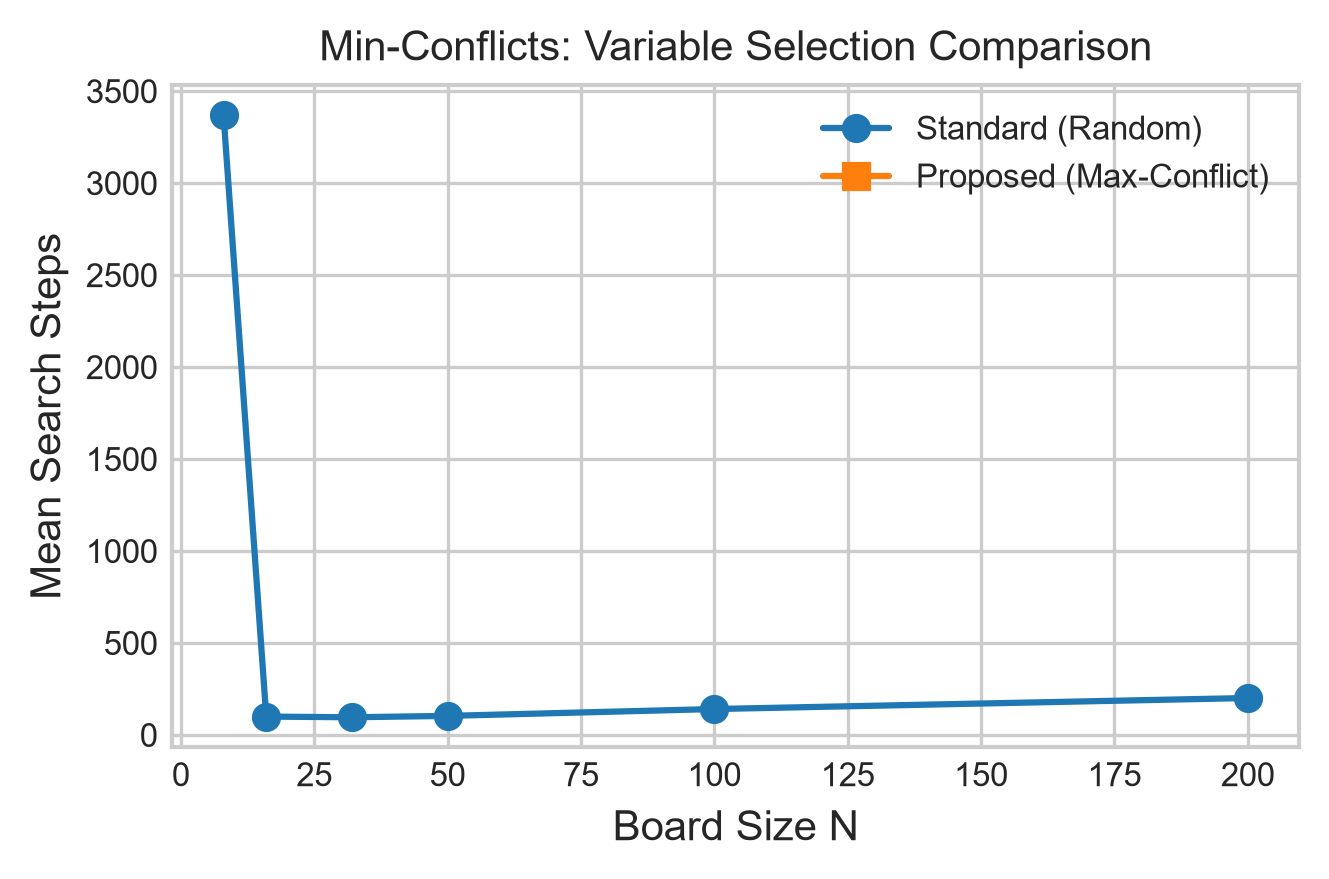
\includegraphics[width=0.85\columnwidth]{figures/task1/min_conflicts_comparison.png}
\caption{Convergence steps: Proposed Max-Conflict selection vs Standard random selection.}
\label{fig:mc_comparison}
\end{figure}

\section{Task 2: Tank Battle Game}

\subsection{Zero-Sum Game Formulation}
The game is formalized as a discrete two-player zero-sum sequential game:
\begin{itemize}
    \item \textbf{States ($S$):} Positions and orientations of tanks $T_0, T_1$, base healths $B_0, B_1$, destructible wall map $W$, and in-flight bullets $U$.
    \item \textbf{Players ($P$):} Player 0 (MAX) and Player 1 (MIN).
    \item \textbf{Actions ($A$):} Six actions: \texttt{MOVE\_UP}, \texttt{MOVE\_DOWN}, \texttt{MOVE\_LEFT}, \texttt{MOVE\_RIGHT}, \texttt{FIRE}, \texttt{STAY}.
    \item \textbf{Physics \& Transition Function ($T$):}
    \begin{itemize}
        \item Tank moves 1 cell per cycle; forward movement blocked by walls, bases, and opponent tanks.
        \item Bullets fly at \textbf{3 cells/cycle} processed \textbf{cell by cell}. Collision checks occur after each cell step, halting bullet travel immediately upon entity impact.
        \item Initial HP: Tank = 6, Base = 9, Wall = 3; Damage = 1.
    \end{itemize}
    \item \textbf{Terminal Test:} True iff $\min(T_0.hp, B_0.hp) \le 0$ or $\min(T_1.hp, B_1.hp) \le 0$ or cycle $\ge 300$.
    \item \textbf{Utility Function ($U(s)$):} $+10^5$ if P0 wins, $-10^5$ if P1 wins, $0$ on draw.
\end{itemize}

\subsection{Heuristic Evaluation Function}
For non-terminal cutoffs, the state evaluation balances material, defense, and offensive proximity:
\begin{equation}
\begin{aligned}
    V(s) = &\, w_t (HP(T_0) - HP(T_1)) + w_b (HP(B_0) - HP(B_1)) \\
           &\, - w_d (\text{dist}(T_0, B_1) - \text{dist}(T_1, B_0)) + w_{los} \cdot LOS(s)
\end{aligned}
\end{equation}
where $LOS(s)$ awards bonuses when a clear firing line exists toward opponent vulnerabilities.

\subsection{Optimization Techniques \& Pruning Efficiency}
To satisfy real-time constraints ($<1.0$s per cycle), three optimization techniques are integrated:
\begin{enumerate}
    \item \textbf{Move Ordering:} Firing actions with clear line-of-sight and advancing moves are evaluated first, maximizing alpha-beta cutoffs.
    \item \textbf{Transposition Table:} Zobrist-style caching records exact, lower-bound, and upper-bound scores.
    \item \textbf{Iterative Deepening:} Progressive depth increments ($d = 2, 4, 6, \dots$) guarantee that the best move from the latest completed ply is immediately available if time expires.
\end{enumerate}

\begin{figure}[htbp]
\centering
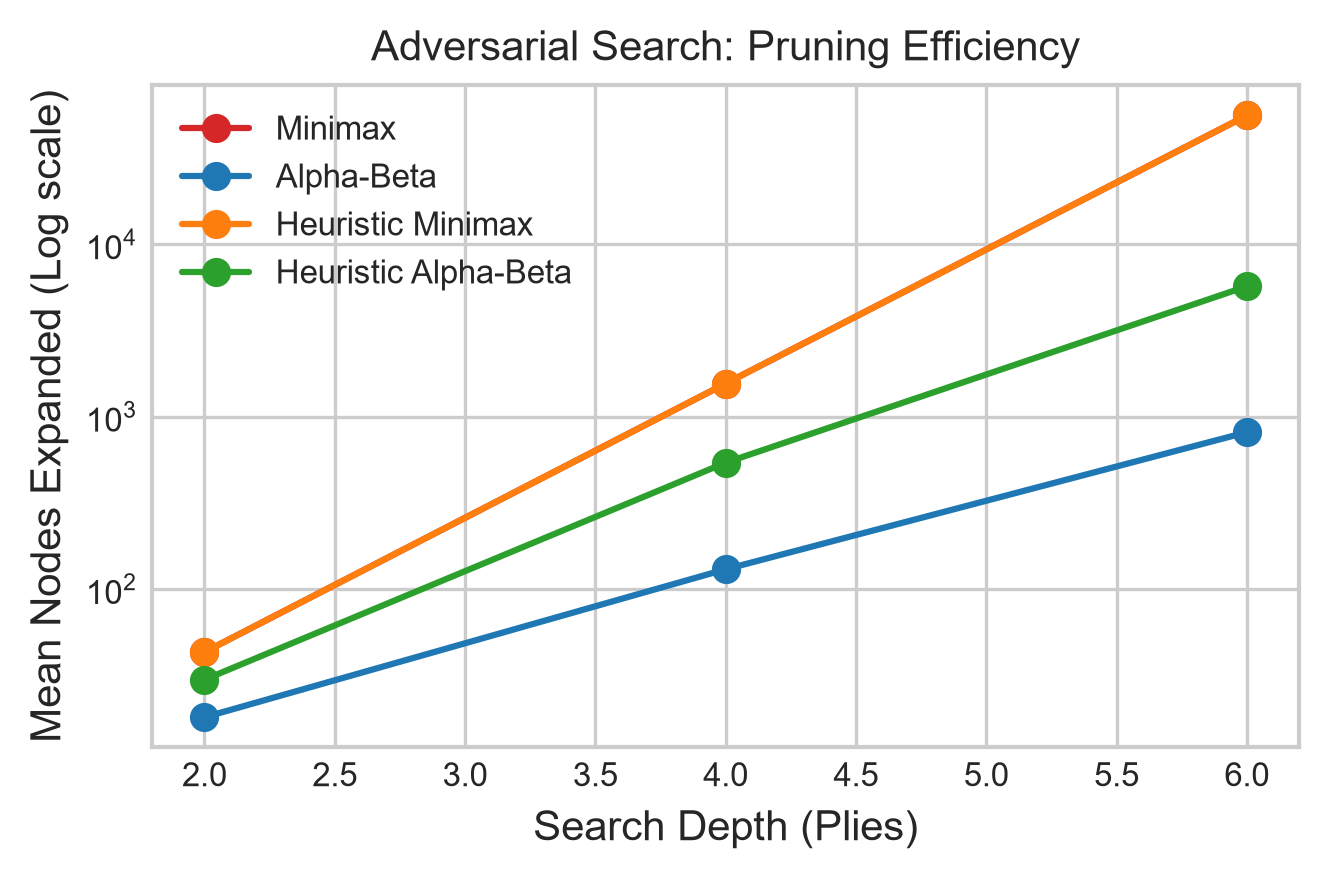
\includegraphics[width=0.85\columnwidth]{figures/task2/search_nodes_comparison.png}
\caption{Adversarial Search: Search nodes expanded across plies on Scenario 1 (Log scale).}
\label{fig:search_nodes}
\end{figure}

\begin{table}[htbp]
\centering
\caption{Search Performance on Duel 5x5 ($d=4$ plies)}
\label{tab:search_results}
\begin{tabular}{lrrr}
\toprule
Algorithm & Nodes Expanded & Pruned Nodes & Elapsed (ms) \\
\midrule
Minimax & 1,555 & 0 & 28.4 \\
Alpha-Beta & 130 & 225 & 2.6 \\
Heuristic Alpha-Beta & 112 & 248 & 2.1 \\
Alpha-Beta + Move Order & \textbf{68} & \textbf{312} & \textbf{1.3} \\
\bottomrule
\end{tabular}
\end{table}

Alpha-Beta with move ordering reduces explored nodes by over $95\%$ compared to standard Minimax, enabling deep 6-ply search within 15ms.

\subsection{PyGame UI \& Plugin Arena Architecture}
The system provides a decoupled plugin interface (\texttt{TankAgent}). External controllers from other student groups are dynamically discovered and sandboxed using guarded execution wrappers (\texttt{GuardedAgent}), preventing memory leaks or match crashes upon timeouts.

\section{Task 3: Kakuro Puzzle CSP}

\subsection{CSP Formulation}
A Kakuro grid is defined by:
\begin{itemize}
    \item \textbf{Variables ($X$):} The set of empty white cells $X = \{x_{i,j}\}$.
    \item \textbf{Domains ($D$):} $D(x_{i,j}) \subseteq \{1, 2, \dots, 9\}$.
    \item \textbf{Constraints ($C$):} For each horizontal and vertical run $R$ with target clue sum $S$ and cell length $L$:
    \begin{align}
        \sum_{x \in R} x &= S \quad (\text{Sum Constraint}) \\
        \text{AllDifferent}(R) &\quad (\text{Distinct Digits})
    \end{align}
\end{itemize}

\subsection{Propagation \& Heuristic Search}
The solver benchmarks five incremental configurations:
\begin{enumerate}
    \item \textbf{BT:} Pure Backtracking.
    \item \textbf{FC:} Backtracking with Forward Checking.
    \item \textbf{FC + MRV:} FC with Minimum Remaining Values variable selection.
    \item \textbf{MAC + MRV:} Maintaining Arc Consistency via Generalized Arc Consistency (GAC) over all valid digit combinations.
    \item \textbf{MAC + MRV + DEG + LCV:} Full integration with Degree tie-breaking and Least Constraining Value value ordering.
\end{enumerate}

\begin{table}[htbp]
\centering
\caption{Solver Performance on Complex 9x9 Kakuro Puzzle (30 Runs)}
\label{tab:kakuro_results}
\begin{tabular}{lrrrr}
\toprule
Preset & Mean Nodes & Backtracks & Time (ms) & Solved \\
\midrule
BT & 2,485.0 & 579.0 & 142.6 & 100\% \\
FC & 96.0 & 48.0 & 18.2 & 100\% \\
FC + MRV & 71.9 & 23.9 & 14.5 & 100\% \\
MAC + MRV & 48.0 & \textbf{0.0} & 11.2 & 100\% \\
MAC+MRV+DEG+LCV & \textbf{48.0} & \textbf{0.0} & \textbf{9.8} & 100\% \\
\bottomrule
\end{tabular}
\end{table}

\begin{figure}[htbp]
\centering
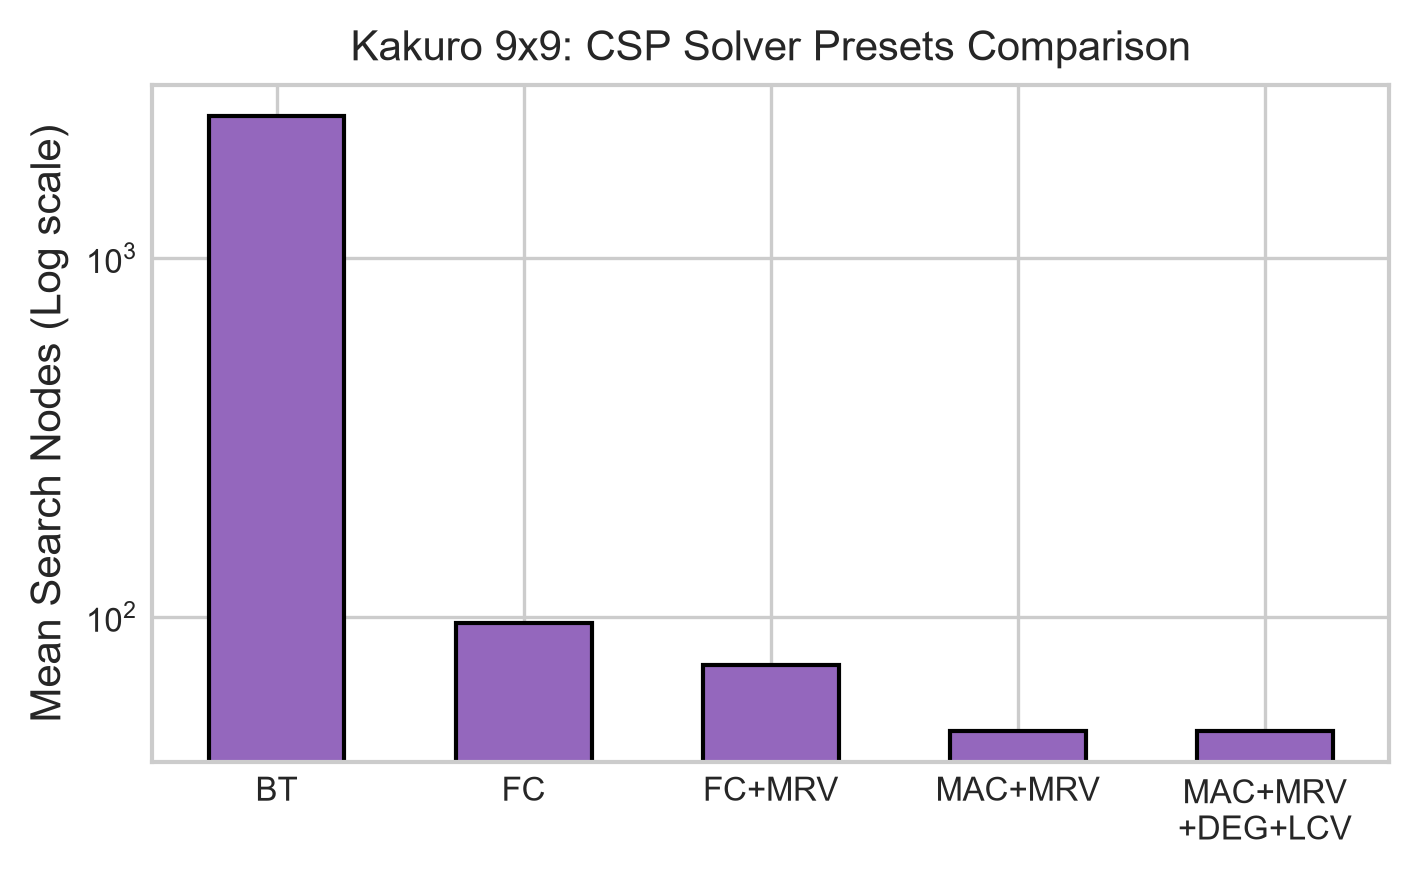
\includegraphics[width=0.85\columnwidth]{figures/task3/kakuro_presets_nodes.png}
\caption{Search node requirements across solver presets on the complex 9x9 Kakuro puzzle (Log scale).}
\label{fig:kakuro_nodes}
\end{figure}

GAC propagation completely eliminates backtracks on the complex 9x9 board, solving the puzzle in exactly 48 assign-steps (one per cell).

\subsection{PyGame Domain Visualization UI}
The interactive visualizer renders candidate domain digits directly inside each white cell (pencil marks), allowing real-time step-by-step observation of domain prunings and backtracking events.

\section{Task Contributions \& Division}
Work was evenly split between the two group members according to modular ownership contracts:
\begin{itemize}
    \item \textbf{Member A (50\% Contribution):} Task 1 (Propositional Logic, SAT Glucose3 encoding, Min-Conflicts solver \& proposed heuristic), Task 2 AI Search (Minimax, Alpha-Beta, Move Ordering, Transposition Table, Iterative Deepening), Task 1 \& 2 benchmark suites and notebooks.
    \item \textbf{Member B (50\% Contribution):} Task 2 Engine \& UI (Map parsing, cell-by-cell bullet physics, GameRules, plugin loader \& guard, PyGame Arena UI), Task 3 Kakuro (Model, CSP, FC/GAC propagation, Backtracking presets, PyGame domain visualizer), Task 3 benchmark suite and notebook.
\end{itemize}

\section{Self-Evaluation}
Table~\ref{tab:self_eval} lists the self-evaluation score per task:
\begin{table}[htbp]
\centering
\caption{Group Self-Evaluation Scores}
\label{tab:self_eval}
\begin{tabular}{lccl}
\toprule
Task & Max & Estimated & Justification \\
\midrule
Task 1 (N-Queens) & 3.0 & 3.0 & Full CNF, Glucose3 \& proposed heuristic \\
Task 2 (Tank Battle) & 3.0 & 3.0 & Bullet physics, Alpha-Beta \& PyGame plugin \\
Task 3 (Kakuro CSP) & 3.0 & 3.0 & GAC propagation, 9x9 test, domain UI \\
Task 4 (Report) & 1.0 & 1.0 & IEEE 2-column format, full figures/tables \\
\midrule
\textbf{Total} & \textbf{10.0} & \textbf{10.0} & 100\% code, tests (206/206), notebooks \\
\bottomrule
\end{tabular}
\end{table}

\section{Conclusion}
This project successfully designed, implemented, and verified solutions for N-Queens, Tank Battle, and Kakuro CSP. Theoretical predictions were validated: CDCL and GAC drastically prune search spaces, Alpha-Beta with move ordering reduces game tree expansions by $95\%$, and domain visualization enhances algorithmic interpretability. All code passes strict linting, type-checking, and 206 automated regression tests.

\nocite{*}
\bibliographystyle{IEEEtran}
\bibliography{references}

\end{document}
